\chapter{Circuiti elettrici e leggi di Kirchhoff}

\begin{concetto}
Questo capitolo introduce i concetti fondamentali della teoria dei circuiti: che cos'è un circuito elettrico, che cosa sono un nodo e una maglia, e come si applicano le due leggi di Kirchhoff per analizzare circuiti semplici. Le leggi di Kirchhoff sono gli strumenti di base per risolvere qualsiasi circuito, dal più semplice al più complesso, e costituiscono il ponte tra i concetti di tensione e corrente introdotti nel capitolo precedente e la risoluzione concreta dei problemi circuitali.
\end{concetto}

\section{Che cos'è un circuito elettrico}

Un \textbf{circuito elettrico} è un insieme di componenti elettrici collegati tra loro in modo da formare un \textbf{percorso chiuso} attraverso il quale può fluire la corrente elettrica. Il percorso chiuso è la condizione essenziale: se il percorso non è chiuso, la corrente non può circolare.

I componenti che si incontrano in un circuito si possono raggruppare in tre categorie fondamentali:

\begin{concetto}
\textbf{Componenti fondamentali di un circuito}
\begin{itemize}[leftmargin=1cm]
  \item i \textbf{generatori}, che mantengono una differenza di potenziale tra i loro terminali e forniscono energia al circuito (pile, batterie, alimentatori);
  \item i \textbf{conduttori}, cioè i fili che collegano tra loro i componenti e permettono il passaggio della corrente;
  \item gli \textbf{utilizzatori}, che assorbono energia elettrica e la trasformano in altre forme di energia (lampadine, resistori, motori).
\end{itemize}
\end{concetto}

Un circuito si dice \textbf{aperto} quando il percorso è interrotto in almeno un punto: in questo caso la corrente non circola. Si dice \textbf{chiuso} quando il percorso è completo: la corrente può circolare. Un interruttore è un dispositivo che permette di aprire o chiudere volontariamente un circuito.

\begin{esempio}
\textbf{La torcia.} Una torcia è un circuito semplicissimo: una pila , due fili, una lampadina e un interruttore. Quando l'interruttore è chiuso, il percorso è completo, la corrente circola e la lampadina si accende. Quando l'interruttore è aperto, il percorso è interrotto e la lampadina si spegne.
\end{esempio}

\begin{attenzione}
In un circuito reale i fili hanno una resistenza piccolissima ma non nulla. Nei circuiti ideali, che sono quelli che si studiano in questa sede, i fili si considerano conduttori perfetti, cioè con resistenza nulla.
\end{attenzione}

\subsection{Il nodo}

In un circuito possono incontrarsi più conduttori nello stesso punto. Questo punto prende il nome di \textbf{nodo}.

\begin{concetto}
Un \textbf{nodo} è un punto del circuito in cui convergono \textbf{tre o più} conduttori. Due soli conduttori che si incontrano non formano un nodo, perché non c'è alcuna suddivisione della corrente: il punto è semplicemente un punto di collegamento tra due componenti in serie.
\end{concetto}

\begin{figure}[htbp]
\centering
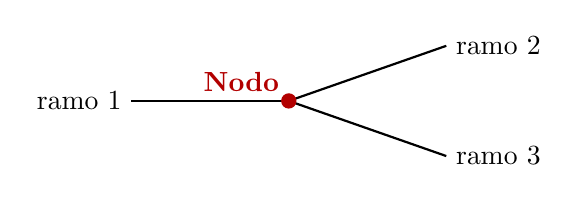
\begin{tikzpicture}[scale=1]
  % Rami che convergono nel nodo
  \draw[thick] (-2,0) -- (0,0);
  \draw[thick] (0,0) -- (2,0.7);
  \draw[thick] (0,0) -- (2,-0.7);
  % Nodo
  \filldraw[red!70!black] (0,0) circle (0.09);
  \node[above left, red!70!black] at (0,0) {\textbf{Nodo}};
  % Etichette dei rami
  \node[left] at (-2,0) {ramo 1};
  \node[right] at (2,0.7) {ramo 2};
  \node[right] at (2,-0.7) {ramo 3};
\end{tikzpicture}
\end{figure}

\begin{esempio}
In un circuito con una pila e due lampadine collegate in parallelo, il polo positivo della pila è collegato a un punto in cui il filo si dirama verso le due lampadine: quel punto è un nodo. Lo stesso vale per il polo negativo.
\end{esempio}

\subsection{La maglia}

Un altro concetto fondamentale è quello di maglia.

\begin{concetto}
Una \textbf{maglia} è un qualsiasi percorso chiuso non intrecciato che parte da un nodo e ritorna allo stesso nodo senza passare due volte per lo stesso ramo. In altre parole, è un anello chiuso all'interno del circuito.
\end{concetto}

Una maglia può contenere al suo interno altri percorsi chiusi oppure no. Quando non ne contiene, si parla di \textbf{maglia elementare}.

\begin{concetto}
Una \textbf{maglia elementare} (o maglia semplice) è una maglia che non contiene al suo interno altre maglie. In pratica, è il più piccolo anello chiuso che si può individuare in un circuito.
\end{concetto}

\begin{attenzione}
Saper distinguere tra maglie elementari e non elementari è importante perché, applicando la legge delle maglie, si scelgono di norma le maglie elementari. Le maglie non elementari danno equazioni che sono combinazione lineare di quelle elementari e non aggiungono informazione.
\end{attenzione}




\section{La legge di Kirchhoff alle Tensioni (legge delle maglie)}

\begin{concetto}
\textbf{LKT (legge delle maglie).} La somma algebrica delle tensioni lungo una maglia è nulla:
\[
\sum_k V_k = 0.
\]
Equivalentemente, la somma delle forze elettromotrici presenti nella maglia è uguale alla somma delle cadute di tensione sui resistori:
\[
\sum \mathcal{E} = \sum R\,I.
\]
\end{concetto}

Questa legge esprime il fatto che, percorrendo un percorso chiuso, si ritorna al punto di partenza con lo stesso potenziale: la somma dei guadagni di tensione deve uguagliare la somma delle perdite.

\subsection{La convenzione dei segni}

Per applicare correttamente la seconda legge di Kirchhoff bisogna fissare una \textbf{convenzione dei segni} e seguirla con coerenza. La procedura è la seguente:

\begin{enumerate}[leftmargin=1cm]
  \item si sceglie arbitrariamente un \textbf{verso di percorrenza} della maglia (orario o antiorario);
  \item per ogni \textbf{generatore} incontrato lungo il percorso, si attribuisce segno \(+\) se si passa dal polo negativo al polo positivo (guadagno di tensione), segno \(-\) se si passa dal polo positivo al polo negativo;
  \item per ogni \textbf{resistore} percorso da una corrente \(I\), si attribuisce segno \(-\) alla caduta \(RI\).
\end{enumerate}

In forma compatta, scrivendo \(\sum V_k = 0\) con questa convenzione, si ottiene direttamente l'equazione risolutiva.

\begin{attenzione}
Il verso di percorrenza scelto è arbitrario: cambiandolo si ottiene un'equazione equivalente, moltiplicata per \(-1\). Il risultato finale non cambia. La cosa importante è non cambiare convenzione a metà calcolo.
\end{attenzione}

\subsection{Esempio di applicazione}

\begin{esempio}
\textbf{Circuito con un solo anello.} Si consideri un circuito formato da una pila con forza elettromotrice \(\mathcal{E} = 12\,[\text{V}]\) e due resistori in serie, \(R_1 = 4\,[\Omega]\) e \(R_2 = 2\,[\Omega]\). Calcolare la corrente che circola nel circuito.

\smallskip
\textbf{Soluzione.} Il circuito ha una sola maglia. Scegliamo come verso di percorrenza quello orario. Percorrendo la maglia:

\begin{itemize}[leftmargin=1cm]
  \item attraverso la pila si passa dal polo negativo al polo positivo: guadagno \(+\mathcal{E}\);
  \item attraverso \(R_1\) la corrente ha lo stesso verso del percorso: caduta \(-R_1 I\);
  \item attraverso \(R_2\) la corrente ha lo stesso verso del percorso: caduta \(-R_2 I\).
\end{itemize}

La seconda legge di Kirchhoff fornisce
\[
\mathcal{E} - R_1 I - R_2 I = 0.
\]
Da cui
\[
I = \frac{\mathcal{E}}{R_1 + R_2} = \frac{12}{4 + 2} = 2\,[\text{A}].
\]
\end{esempio}

\subsection{Esempio con più generatori}

\begin{esempio}
\textbf{Circuito con due generatori.} Si consideri una maglia singola formata da:
\begin{itemize}[leftmargin=1cm]
  \item due generatori \(\mathcal{E}_1 = 12\,[\text{V}]\) e \(\mathcal{E}_2 = 6\,[\text{V}]\);
  \item due resistori, \(R_1 = 3\,[\Omega]\) e \(R_2 = 1\,[\Omega]\).
\end{itemize}
I due generatori sono disposti in modo che \(\mathcal{E}_1\) favorisca la corrente nel verso orario, mentre \(\mathcal{E}_2\) si opponga. Calcolare la corrente \(I\) che circola nella maglia.

\smallskip
\textbf{Soluzione.} Scegliamo come verso di percorrenza quello orario. Rappresentiamo la maglia e indichiamo con frecce le tensioni incontrate lungo il percorso.



\begin{center}
\begin{tikzpicture}[scale=1]
  % --- Maglia rettangolare con interruzioni per i resistori ---
  % Lato sinistro (generatore 1): linea continua
  \draw[thick] (0,0) -- (0,3);
  % Lato destro (generatore 2): linea continua
  \draw[thick] (6,0) -- (6,3);
  % Lato superiore: interrotto al centro per R1
  \draw[thick] (0,3) -- (2,3);
  \draw[thick] (4,3) -- (6,3);
  % Lato inferiore: interrotto al centro per R2
  \draw[thick] (0,0) -- (2,0);
  \draw[thick] (4,0) -- (6,0);

  % --- Generatore 1 (lato sinistro, + in alto) ---
  % Sostituisci: \generatore[0]{0}{1.5}{}
\generatore[rot=0]{0}{1.5}
\generatore[rot=0]{6}{1.5}

  % --- Resistore R1 (lato superiore) ---
  % Sostituisci: \resistoreANSI[0]{3}{3}{}
\resistoreANSI[rot=0, label = $R_1$, label dy = -0.5]{3}{3}
\resistoreANSI[rot=0, label = $R_2$, label dy = 0.5]{3}{0}

  % --- Frecce per le tensioni (all'esterno della maglia) ---

  % Generatore 1: dal basso verso l'alto (guadagno +E1)
  \draw[->, thick, rossoscuro] (-0.6,0.5) -- (-0.6,2.5);
  \node[left, rossoscuro] at (-0.6,1.5) {\(+\mathcal{E}_1\)};

  % Generatore 2: dal basso verso l'alto (guadagno +E2)
  \draw[->, thick, rossoscuro] (6.6,0.5) -- (6.6,2.5);
  \node[right, rossoscuro] at (6.6,1.5) {\(+\mathcal{E}_2\)};

  % Resistore R1: verso orario (da sinistra a destra)
  \draw[->, thick, blue] (4,3.6) -- (2,3.6);
  \node[above, blue] at (3,3.6) {\(V_1\)};

  % Resistore R2: verso orario (da destra a sinistra)
  \draw[->, thick, blue] (2,-0.6) -- (4,-0.6);
  \node[below, blue] at (3,-0.6) {\(V_2\)};

  % Verso di percorrenza orario (freccia curva al centro)
  \draw[->, thick, green!60!black] (1.8,0.9) arc (170:10:1.2);
  \node[green!60!black] at (3,1.2) {verso orario};
\end{tikzpicture}
\end{center}







Percorrendo la maglia in verso orario:
\begin{itemize}[leftmargin=1cm]
  \item attraverso \(\mathcal{E}_1\) si passa dal polo negativo al polo positivo: guadagno \(+\mathcal{E}_1\);
  \item attraverso \(R_1\) e \(R_2\): caduta \(V_1 = -R_1 I\) e \(V_2 = -R_2 I\);
  \item attraverso \(\mathcal{E}_2\) si passa dal polo positivo al polo negativo: guadagno \(-\mathcal{E}_2\);
\end{itemize}

La legge di Kirchhoff alle Tensioni (LKT) fornisce:
\[
\mathcal{E}_1 - V_1 - \mathcal{E}_2 - V_2 = 0 \qquad\Longrightarrow\qquad
\mathcal{E}_1 - R_1 I - \mathcal{E}_2 - R_2 I = 0.
\]
Sostituendo i valori:
\[
12 - 3I - 6 - 1I = 0
\quad\Rightarrow\quad
6 - 4I = 0
\quad\Rightarrow\quad
I = \frac{6}{4} = 1.5\,[\text{A}].
\]
La corrente positiva indica che il verso effettivo è quello orario, cioè quello scelto.
\end{esempio}

\begin{curiosita}
Le leggi di Kirchhoff valgono per qualsiasi circuito, indipendentemente dal numero di componenti. Anche i circuiti integrati più complessi, con miliardi di transistori, vengono analizzati con gli stessi due principi. La potenza del metodo sta nella sua semplicità: due leggi, applicate con coerenza, bastano per risolvere qualsiasi rete lineare.
\end{curiosita}





\section{La legge di Kirchhoff alle Correnti (legge dei nodi)}
\begin{concetto}
\textbf{LKC (legge dei nodi).} In un nodo, la somma delle correnti che entrano è uguale alla somma delle correnti che escono:
\[
\sum I_{\text{entranti}} = \sum I_{\text{uscenti}}.
\]
Equivalentemente, attribuendo segno positivo alle correnti entranti e negativo a quelle uscenti (o viceversa), la somma algebrica di tutte le correnti che confluiscono in un nodo è nulla:
\[
\sum_k I_k = 0.
\]
\end{concetto}

Questa legge esprime un principio di conservazione: la carica elettrica non può accumularsi in un nodo né sparire, quindi tanta carica entra quanta esce nell'unità di tempo.

\begin{esempio}
\textbf{Nodo con tre rami.} In un nodo convergono tre conduttori. Nel primo entra una corrente \(I_1 = 3\,[\text{A}]\), nel secondo entra una corrente \(I_2 = 1\,[\text{A}]\). Quanta corrente esce dal terzo ramo?

\smallskip
\textbf{Soluzione.} Applichiamo la legge dei nodi:
\[
I_1 + I_2 = I_3 \quad \Longrightarrow \quad I_3 = 3 + 1 = 4\,[\text{A}].
\]
Dal terzo ramo escono \(4\,[\text{A}]\).
\end{esempio}

\begin{esempio}
\textbf{Nodo con quattro rami.} In un nodo entrano \(I_1 = 5\,[\text{A}]\) e \(I_2 = 2\,[\text{A}]\), mentre escono \(I_3 = 3\,[\text{A}]\) e \(I_4\) incognita. Determinare \(I_4\).

\smallskip
\textbf{Soluzione.}
\[
I_1 + I_2 = I_3 + I_4 \quad \Longrightarrow \quad 5 + 2 = 3 + I_4 \quad \Longrightarrow \quad I_4 = 4\,[\text{A}].
\]
\end{esempio}


\section{La massa}

\begin{concetto}
La \textbf{massa} (in inglese \textit{ground}, spesso indicata con il simbolo \(\bot\) o GND) è un \textbf{punto di riferimento} del circuito al quale si attribuisce per convenzione il potenziale elettrico \(V = 0\,[\text{V}]\). Tutti gli altri potenziali del circuito vengono misurati rispetto a questo punto.
\end{concetto}

\subsection{Perché serve un riferimento}

Una tensione non è mai un valore assoluto: è sempre una \textbf{differenza di potenziale tra due punti}. Dire ``in questo punto c'è una tensione di \(5\,[\text{V}]\)'' non ha senso se non si specifica \emph{rispetto a che cosa}.

Per capirlo, si può pensare all'altezza. Se si dice ``sono alto \(10\,[\text{m}]\)'', la frase è ambigua: \(10\,[\text{m}]\) rispetto a cosa? Se ci si trova al secondo piano di un palazzo, l'altezza rispetto al pavimento del piano è circa \(1{,}7\,[\text{m}]\), mentre l'altezza rispetto al livello del mare è molto maggiore. L'``altezza'' cambia a seconda del \textbf{riferimento} scelto. Eppure la posizione fisica è sempre la stessa: quello che cambia è solo il numero usato per descriverla.

Lo stesso vale per il potenziale elettrico. In un circuito, il potenziale di un nodo non ha un valore assoluto: ha senso solo se confrontato con un altro nodo. Per evitare di dover specificare ogni volta ``rispetto a questo nodo'', si sceglie un nodo di riferimento e lo si chiama \textbf{massa}. A quel nodo si assegna \(V = 0\,[\text{V}]\), e tutti gli altri potenziali si misurano rispetto a lui.

\begin{esempio}
\textbf{L'analogia del palazzo.}
\begin{itemize}[leftmargin=1cm]
  \item Il \textbf{pavimento del piano} è come la massa: è il livello rispetto al quale si misurano tutte le altezze dentro quell'appartamento.
  \item L'altezza di una persona (\(1{,}7\,[\text{m}]\)) è come la tensione di un nodo rispetto alla massa.
  \item Cambiando appartamento e prendendo come riferimento un altro pavimento, i numeri cambiano, ma la posizione fisica no.
  \item La differenza di altezza tra due persone (per esempio \(20\,[\text{cm}]\)) è come una \textbf{differenza di potenziale}: è quella che conta davvero, e non dipende dal riferimento scelto.
\end{itemize}
\end{esempio}

\subsection{Che cosa cambia e che cosa no}

\begin{itemize}[leftmargin=1cm]
  \item \textbf{Cambia} il valore numerico dei potenziali: spostando la massa in un altro punto, tutti i potenziali cambiano dello stesso valore.
  \item \textbf{Non cambiano} le \textbf{differenze di potenziale} tra i nodi, cioè le tensioni che compaiono nelle leggi di Kirchhoff e nella legge di Ohm.
  \item \textbf{Non cambiano} le correnti, perché esse dipendono solo dalle differenze di potenziale.
\end{itemize}

Per questo la scelta della massa è \textbf{arbitraria}: il funzionamento del circuito non dipende da dove viene messa. È solo una convenzione comoda, che permette di parlare di ``potenziale di un nodo'' senza specificare ogni volta rispetto a che cosa.

\begin{attenzione}
La massa \textbf{non è} un componente che ``assorbe'' corrente o che ``scarica'' la corrente a terra. È solo un'\textbf{etichetta} che indica: ``questo nodo è il riferimento, il suo potenziale vale \(0\,[\text{V}]\)''. Nei circuiti reali la massa è spesso collegata allo chassis metallico del dispositivo o alla terra vera e propria (impianto di terra), ma concettualmente è solo un punto scelto come riferimento.
\end{attenzione}

\subsection{Il simbolo}

Nei circuiti la massa si rappresenta con un simbolo formato da tre linee orizzontali di lunghezza decrescente, oppure con un triangolino. Il filo che arriva al simbolo indica il nodo scelto come riferimento.

\begin{center}
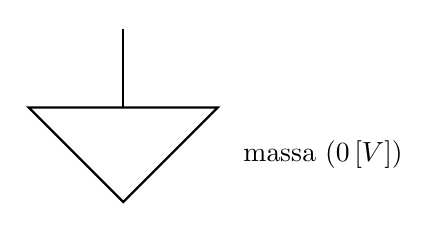
\begin{tikzpicture}[scale=2]
  % Filo
  \draw[thick] (0,0) -- (0,-0.5);
  % Triangolo
  \draw[thick] (-0.6,-0.5) -- (0.6,-0.5) -- (0,-1.1) -- cycle;
  % Etichetta
  \node[right] at (0.7,-0.8) {massa (\(0\,[\text{V}]\))};
\end{tikzpicture}
\end{center}


\begin{curiosita}
Nella maggior parte dei circuiti elettronici la massa è il nodo con più connessioni: è il ``filo comune'' a cui fanno riferimento tutti i segnali. Nei telefoni, nei computer e in quasi tutti i dispositivi elettronici, la massa è il punto rispetto al quale si misura ogni tensione. Senza un riferimento comune, parlare di ``\(3{,}3\,[\text{V}]\)'' o ``\(5\,[\text{V}]\)'' non avrebbe alcun significato.
\end{curiosita}
















\section{Partitore di tensione}

\begin{concetto}
Il \textbf{partitore di tensione} è un circuito formato da due o più resistori in serie. Esso permette di ottenere, ai capi di un resistore, una frazione della tensione totale applicata. È una conseguenza della legge di Ohm e della legge di Kirchhoff alle tensioni.
\end{concetto}

\subsection{Circuito con due resistori in serie}

Si consideri una serie di due resistori \(R_1\) e \(R_2\) alimentata da una tensione \(V_{\text{in}}\). La tensione di uscita \(V_{\text{out}}\) è prelevata ai capi di \(R_2\). Il terminale negativo del generatore è collegato alla \textbf{massa}, cioè al nodo di riferimento a cui si attribuisce \(V = 0\,[\text{V}]\).

\begin{center}
\begin{tikzpicture}[scale=1]
  % Filo sinistro dal basso al generatore
  \draw[thick] (0,0) -- (0,1.2);
  % Generatore
  \generatore{0}{2}{}
  \draw node[left] at (-0.5,2) {\(V_{\text{in}}\)};
  % Filo dal generatore al lato superiore
  \draw[thick] (0,2.8) -- (0,4);
  % Filo superiore fino al resistore R1
  \draw[thick] (0,4) -- (1,4);
  % Resistore R1
  \resistoreANSI[label = $R_1$, label dy = -0.5]{2}{4}
  \resistoreANSI[rot = 90, label = $R_2$, label dx = -0.6, label dy = 0]{4}{2}
  
  \draw[thick] (3,4) -- (4,4);
  \draw[thick] (4,4) -- (4,3);
  \draw[thick] (4,1) -- (4,0);
  \draw[thick] (4,0) -- (0,0);

  \massa{4}{0}

  \draw[thick] (4,0) -- (4.5,0);
  \draw[thick] (4,4) -- (4.5,4);
  \draw[thick] (4.6,4) circle (0.1);
  \draw[thick] (4.6,0) circle (0.1);
  % Etichetta V_out
  \draw[->, thick, red] (4.7,0.5) -- (4.7,3.5) node[midway,right] {\(V_{\text{out}}\)};
\end{tikzpicture}
\end{center}

\paragraph{Dimostrazione.}
Poiché \(R_1\) e \(R_2\) sono in serie, sono percorsi dalla stessa corrente \(I\). Applicando la legge di Kirchhoff alle tensioni all'unica maglia:

\[
V_{\text{in}} = V_{R_1} + V_{R_2}.
\]

Per la legge di Ohm:

\[
V_{R_1} = R_1 I, \qquad V_{R_2} = R_2 I.
\]

Sostituendo:

\[
V_{\text{in}} = R_1 I + R_2 I = (R_1 + R_2) I.
\]

Da cui la corrente:

\[
I = \frac{V_{\text{in}}}{R_1 + R_2}.
\]

La tensione ai capi di \(R_2\) è:

\[
V_{\text{out}} = V_{R_2} = R_2 I = R_2 \frac{V_{\text{in}}}{R_1 + R_2}.
\]

Quindi la formula del partitore di tensione è:

\[
\boxed{
V_{\text{out}} = V_{\text{in}} \frac{R_2}{R_1 + R_2}
}
\]

Analogamente, la tensione ai capi di \(R_1\) sarebbe \(V_{R_1} = V_{\text{in}} \frac{R_1}{R_1 + R_2}\).

\paragraph{Proprietà.}
Il resistore più grande ha ai suoi capi la tensione maggiore.
\subsection{Esempio numerico}

Un partitore di tensione ha \(V_{\text{in}} = 12\,[\text{V}]\), \(R_1 = 4\,[\Omega]\), \(R_2 = 2\,[\Omega]\). Calcolare \(V_{\text{out}}\) ai capi di \(R_2\).

\[
V_{\text{out}} = 12 \cdot \frac{2}{4+2} = 12 \cdot \frac{2}{6} = 4\,[\text{V}].
\]

\section{Partitore di corrente}

\begin{concetto}
Il \textbf{partitore di corrente} è un circuito formato da due o più resistori in parallelo. Esso permette di dividere una corrente totale in più rami. La corrente in ciascun ramo è inversamente proporzionale alla resistenza del ramo stesso.
\end{concetto}

\subsection{Circuito con due resistori in parallelo}

Si considerino due resistori \(R_1\) e \(R_2\) collegati in parallelo, alimentati da una corrente totale \(I_{\text{tot}}\). La corrente si divide nei due rami in \(I_1\) e \(I_2\). Il nodo inferiore destro è collegato alla \textbf{massa}, cioè al riferimento a cui si attribuisce \(V = 0\,[\text{V}]\).

\begin{center}
\begin{tikzpicture}[scale=1]
  % Rail superiore
  \draw[thick] (0,4) -- (4,4);
  % Rail inferiore
  \draw[thick] (0,0) -- (4,0);

  % Ramo sinistro con generatore
  \draw[thick] (0,0) -- (0,1.2);
  \generatore{0}{2}
  \draw[thick] (0,2.8) -- (0,4);

  % Ramo con R1 (verticale, x=2)
  \draw[thick] (2,4) -- (2,3);
  \resistoreANSI[rot=90, label=$R_1$, label dx = 0.5, label dy = 0]{2}{2}
  \draw[thick] (2,1) -- (2,0);

  % Ramo con R2 (verticale, x=4)
  \draw[thick] (4,4) -- (4,3);
  \resistoreANSI[rot=90, label=$R_2$, label dx = 0.5, label dy = 0]{4}{2}
  \draw[thick] (4,1) -- (4,0);

  % Corrente totale sul rail superiore
  \draw[->, thick, rossoscuro] (0.5,4.25) -- (1.5,4.25) node[midway,above] {\(I_{\text{tot}}\)};

  % Correnti nei rami (verso il basso)
  \draw[->, thick, bluscuro] (2,3.7) -- (2,3.1) node[midway,right] {\(I_1\)};
  \draw[->, thick, bluscuro] (4,3.7) -- (4,3.1) node[midway,right] {\(I_2\)};

  % Nodi (punti di biforcazione)
  \filldraw (2,4) circle (0.05);
  \filldraw (4,4) circle (0.05);
  \filldraw (2,0) circle (0.05);
  \filldraw (4,0) circle (0.05);

  % Massa
  \massa{3}{0}
\end{tikzpicture}
\end{center}

\paragraph{Dimostrazione.}
Poiché \(R_1\) e \(R_2\) sono in parallelo, ai loro capi c'è la stessa tensione \(V\), misurata rispetto alla massa. Per la legge di Kirchhoff alle correnti applicata al nodo di ingresso:

\[
I_{\text{tot}} = I_1 + I_2.
\]

Per la legge di Ohm:

\[
I_1 = \frac{V}{R_1}, \qquad I_2 = \frac{V}{R_2}.
\]

Sostituendo:

\[
I_{\text{tot}} = \frac{V}{R_1} + \frac{V}{R_2} = V \left( \frac{1}{R_1} + \frac{1}{R_2} \right) = V\, \frac{R_1 + R_2}{R_1 R_2}.
\]

Quindi:

\[
I_{\text{tot}} = V \frac{R_1 + R_2}{R_1 R_2} \quad\Longrightarrow\quad V = I_{\text{tot}} \frac{R_1 R_2}{R_1 + R_2}.
\]

Ora si calcolano le correnti nei due rami:

\[
I_1 = \frac{V}{R_1} = \frac{1}{R_1} I_{\text{tot}} \frac{R_1 R_2}{R_1 + R_2} = I_{\text{tot}} \frac{R_2}{R_1 + R_2}.
\]

\[
I_2 = \frac{V}{R_2} = \frac{1}{R_2} I_{\text{tot}} \frac{R_1 R_2}{R_1 + R_2} = I_{\text{tot}} \frac{R_1}{R_1 + R_2}.
\]

Pertanto le formule del partitore di corrente sono:

\[
\boxed{
I_1 = I_{\text{tot}} \frac{R_2}{R_1 + R_2}
}
\qquad
\boxed{
I_2 = I_{\text{tot}} \frac{R_1}{R_1 + R_2}
}
\]

\paragraph{Proprietà.}
\begin{itemize}[leftmargin=1cm]
  \item La corrente si ripartisce in proporzione inversa alle resistenze: \(\frac{I_1}{I_2} = \frac{R_2}{R_1}\).
  \item Il ramo con resistenza maggiore è percorso da corrente minore.
\end{itemize}

\subsection{Esempio numerico}

Un partitore di corrente ha \(I_{\text{tot}} = 6\,[\text{A}]\), \(R_1 = 2\,[\Omega]\), \(R_2 = 4\,[\Omega]\). Calcolare \(I_1\) e \(I_2\).

\[
I_1 = 6 \cdot \frac{4}{2+4} = 6 \cdot \frac{4}{6} = 4\,[\text{A}],
\]

\[
I_2 = 6 \cdot \frac{2}{2+4} = 6 \cdot \frac{2}{6} = 2\,[\text{A}].
\]

Verifica: \(I_1 + I_2 = 4 + 2 = 6\,[\text{A}] = I_{\text{tot}}\).



\section{Esercizi}

\subsection{Domande di comprensione}

\begin{enumerate}[leftmargin=1cm]
  \item Che cos'è un circuito elettrico e perché deve essere chiuso perché la corrente circoli?
  \item Quali sono i tre tipi di componenti fondamentali di un circuito? Fai un esempio per ciascuno.
  \item Che cos'è un nodo? Perché due soli conduttori che si incontrano non formano un nodo?
  \item Che cos'è una maglia? Che differenza c'è tra maglia e maglia elementare?
  \item Enuncia la prima legge di Kirchhoff e spiega il significato fisico.
  \item Enuncia la seconda legge di Kirchhoff e spiega il significato fisico.
  \item Qual è la convenzione dei segni da usare nella legge delle maglie? Perché è importante non cambiarla a metà calcolo?
  \item Perché, applicando la legge delle maglie, conviene scegliere le maglie elementari?
  \item Quante equazioni indipendenti si possono scrivere ai nodi di un circuito con \(n\) nodi? E quante alle maglie?
\end{enumerate}

\subsection{Esercizi sui nodi}

\begin{esercizio}
\textbf{Esercizio svolto.} In un nodo convergono quattro conduttori. Entrano \(I_1 = 4\,[\text{A}]\) e \(I_2 = 3\,[\text{A}]\); esce \(I_3 = 5\,[\text{A}]\). Calcolare la corrente \(I_4\) nel quarto ramo.

\smallskip
\textbf{Soluzione.} Applichiamo la prima legge di Kirchhoff:
\[
I_1 + I_2 = I_3 + I_4.
\]
Sostituendo i valori:
\[
4 + 3 = 5 + I_4 \quad \Longrightarrow \quad I_4 = 2\,[\text{A}].
\]
La corrente \(I_4\) esce dal nodo.
\end{esercizio}

\textbf{Esercizi da svolgere.}

\begin{enumerate}[leftmargin=1cm]
  \item In un nodo entrano \(I_1 = 6\,[\text{A}]\) e \(I_2 = 2\,[\text{A}]\), ed esce \(I_3 = 5\,[\text{A}]\). Calcolare la corrente nel quarto ramo e stabilirne il verso.
  \item In un nodo convergono cinque rami: entrano \(I_1 = 3\,[\text{A}]\), \(I_2 = 4\,[\text{A}]\), \(I_3 = 1\,[\text{A}]\); esce \(I_4 = 2\,[\text{A}]\). Calcolare \(I_5\).
  \item In un nodo entrano tre correnti: \(I_1 = 1{,}5\,[\text{A}]\), \(I_2 = 2{,}5\,[\text{A}]\), \(I_3 = 3\,[\text{A}]\). Escono due correnti: \(I_4 = 4\,[\text{A}]\) e \(I_5\). Calcolare \(I_5\).
  \item In un nodo la somma delle correnti entranti è \(10\,[\text{A}]\). Se le correnti uscenti sono tre e valgono \(I_1 = 2\,[\text{A}]\), \(I_2 = 3\,[\text{A}]\), calcolare \(I_3\).
  \item In un nodo entrano \(I_1 = 2\,[\text{A}]\) e \(I_2 = 3\,[\text{A}]\), mentre esce \(I_3 = 7\,[\text{A}]\). È possibile? Giustifica la risposta.
\end{enumerate}

\subsection{Esercizi sulle maglie}

\begin{esercizio}
\textbf{Esercizio svolto.} In una maglia sono presenti una pila con \(\mathcal{E} = 9\,[\text{V}]\) e tre resistori in serie, \(R_1 = 1\,[\Omega]\), \(R_2 = 2\,[\Omega]\), \(R_3 = 3\,[\Omega]\). Calcolare la corrente che circola.

\smallskip
\textbf{Soluzione.} Applichiamo la seconda legge di Kirchhoff scegliendo come verso di percorrenza quello orario:
\[
\mathcal{E} - R_1 I - R_2 I - R_3 I = 0.
\]
Da cui
\[
I = \frac{\mathcal{E}}{R_1 + R_2 + R_3} = \frac{9}{1 + 2 + 3} = 1{,}5\,[\text{A}].
\]
\end{esercizio}

\textbf{Esercizi da svolgere.}

\begin{enumerate}[leftmargin=1cm]
  \item In una maglia ci sono una pila da \(6\,[\text{V}]\) e due resistori in serie da \(1\,[\Omega]\) e \(2\,[\Omega]\). Calcolare la corrente.
  \item In una maglia ci sono una pila da \(12\,[\text{V}]\) e tre resistori in serie da \(2\,[\Omega]\), \(3\,[\Omega]\) e \(5\,[\Omega]\). Calcolare la corrente.
  \item In una maglia ci sono due pile in serie, \(\mathcal{E}_1 = 4{,}5\,[\text{V}]\) e \(\mathcal{E}_2 = 1{,}5\,[\text{V}]\), e un resistore \(R = 3\,[\Omega]\). Calcolare la corrente.
  \item In una maglia ci sono una pila da \(9\,[\text{V}]\), un resistore \(R_1 = 2\,[\Omega]\) e un resistore incognito \(R_2\). Se la corrente vale \(1{,}5\,[\text{A}]\), calcolare \(R_2\).
  \item In una maglia circola una corrente di \(0{,}5\,[\text{A}]\). La pila ha una fem di \(6\,[\text{V}]\). Calcolare la resistenza totale del circuito.
\end{enumerate}

\subsection{Esercizi combinati (nodi e maglie)}

\begin{esercizio}
\textbf{Esercizio svolto.} Si consideri un circuito con due maglie elementari. Nel ramo di sinistra c'è una pila \(\mathcal{E}_1 = 10\,[\text{V}]\) e un resistore \(R_1 = 2\,[\Omega]\). Nel ramo centrale c'è un resistore \(R_2 = 4\,[\Omega]\). Nel ramo di destra c'è una pila \(\mathcal{E}_2 = 4\,[\text{V}]\) e un resistore \(R_3 = 2\,[\Omega]\). Le due pile hanno il polo positivo rivolto verso l'alto.

\smallskip
\textbf{Soluzione.} Si scelgono i versi delle correnti e si scrivono le equazioni. Applicando la legge dei nodi al nodo superiore e la legge delle maglie alle due maglie elementari, si ottiene un sistema di tre equazioni in tre incognite. La risoluzione fornisce i valori delle tre correnti. Se una corrente risulta negativa, il verso reale è opposto a quello scelto inizialmente.
\end{esercizio}

\textbf{Esercizi da svolgere.}

\begin{enumerate}[leftmargin=1cm]
  \item Un circuito ha due maglie elementari. Nella maglia di sinistra c'è una pila \(\mathcal{E}_1 = 12\,[\text{V}]\) e un resistore \(R_1 = 3\,[\Omega]\); nella maglia di destra c'è una pila \(\mathcal{E}_2 = 6\,[\text{V}]\) e un resistore \(R_3 = 3\,[\Omega]\); nel ramo centrale c'è un resistore \(R_2 = 6\,[\Omega]\). Calcolare le correnti nei tre rami.
  \item Un circuito ha due maglie elementari. Nella maglia di sinistra c'è una pila \(\mathcal{E}_1 = 9\,[\text{V}]\) e un resistore \(R_1 = 1\,[\Omega]\); nella maglia di destra c'è una pila \(\mathcal{E}_2 = 3\,[\text{V}]\) e un resistore \(R_3 = 2\,[\Omega]\); nel ramo centrale c'è un resistore \(R_2 = 3\,[\Omega]\). Calcolare le correnti nei tre rami.
  \item In un circuito con due maglie elementari, il ramo centrale è percorso da una corrente \(I_2 = 0{,}5\,[\text{A}]\). Se la corrente nella maglia di sinistra è \(I_1 = 1\,[\text{A}]\), calcolare la corrente nella maglia di destra \(I_3\).
  \item Un circuito ha tre resistori in parallelo collegati a una pila. Quanti nodi ha? Quante maglie elementari? 
\end{enumerate}